\section{Marco teórico}
\subsection{Sitios de CQA}
\begin{frame}
	\frametitle{Sitios de CQA}
	\begin{tcolorbox}[colback=blue!5,colframe=blue!40!black,title=Sitios de Community Question Answering]
		Los sitios de \textit{Community Question Answering} CQA, son un tipo especial de sitios web de \textit{Question Answering} (QA), los cuales permiten a los usuarios registrados responder a preguntas formuladas por otras personas.
	\end{tcolorbox}
\end{frame}

\subsection{Sistemas de recomendación}
\begin{frame}
	\frametitle{Sistemas de Recomendación}
	\begin{tcolorbox}[colback=blue!5,colframe=blue!40!black,title=Sistemas de Recomendación]
		Un RS es un conjunto de herramientas de software que sugiere ítems a un usuario, quien posiblemente utilizará algunos de ellos.
	\end{tcolorbox}

	\bigskip
	\begin{itemize}
		\item
		\textbf{Ejemplos}
		\begin{itemize} [<*>]
			\item Recomendación de preguntas similares en el sitio web Quora.
			\item Sitios conocidos como Netflix o Amazon.
		\end{itemize}

		\bigskip

		\item
		\textbf{Funciones de un Sistema de Recomendación}
		\begin{itemize} [<*>]
			\item Aumentar el ratio de conversión en un sitio o aplicación.
			\begin{scriptsize}
				\begin{itemize} [<*>]
					\item Aumentar la cantidad de productos que usuario compra en Amazon, sobre la cantidad de visualizados.
				\end{itemize}
			\end{scriptsize}
			\item Aumentar satisfacción y fidelidad del usuario.
			\begin{itemize} [<*>]
				\item Una mejor experiencia de usuario provoca que los mismos vuelvan al sitio.
			\end{itemize}
		\end{itemize}
	\end{itemize}
\end{frame}

\subsection{Big Data y Arquitecturas}
\begin{frame}
	\frametitle{Big Data}
		\begin{tcolorbox}[colback=blue!5,colframe=blue!40!black,title=Big Data]
			``Conjuntos de datos cuyo tamaño está más allá de la habilidad de las herramientas software de base de datos para capturar, almacenar, gestionar y analizar los datos'' (Manyika et al., 2011).

			\bigskip

			``Big Data son activos de información caracterizados por su alto volumen, velocidad y variedad que demandan formas innovadoras y rentables de procesamiento de información para mejorar la compresión y la toma de decisiones'' (consultora Gartner).
		\end{tcolorbox}
		\bigskip

		\begin{center}
			Se necesitan \textbf{herramientas de software} que nos permitan procesar este volumen de información de manera eficiente y eficaz.
		\end{center}
\end{frame}

\subsection{Medidas de distancia de texto}
\begin{frame}
	\frametitle{Similaridad}
	Las medidas de similaridad son de interés para poder cuantificar la relación entre objetos.
	\bigskip
	\begin{itemize}
		\item
		La función de similaridad es definida satisfaciendo las condiciones:
		\begin{enumerate}[<*>]
			\item Simetría,
			\[S(x_i,x_j)=S(x_j,x_i);\]

			\item Positividad,
			\[0 \leq S(x_i,x_j) \leq 1, \quad \forall x_i,x_j.\]
		\end{enumerate}
		\medskip
		Es posible transformar una medida de similaridad \(S(x_i,x_j)\) en una de distancia \(D(xi,xj)\) que cumpla \(0 \leq D(x_i,x_j) \leq 1\), en el intervalo \([0,1]\). Aplicando \(D(x_i,x_j) = 1 - S(x_i,x_j)\). En este trabajo se utiliza una \textbf{definición relajada de distancia}.

		\bigskip

		\item Se utilizan dos tipos de medidas de similaridad en este trabajo:
		\begin{enumerate}[<*>]
			\item Basadas en espacios vectoriales.
			\item Basadas en taxonomías.
		\end{enumerate}
	\end{itemize}
\end{frame}

\begin{frame}
	\frametitle{Modelo de espacio vectorial}
	En el modelo de \textit{espacio vectorial}, un texto es representado como un vector de términos. Si las palabras son elegidas como términos, entonces cada palabra del vocabulario sería una \textit{dimensión} independiente en el espacio vectorial (Singhal et al., 2001).

	\bigskip

	Típicamente, el ángulo entre los dos vectores es usado como medida de divergencia entre los mismos, y el coseno del ángulo es usado como similaridad numérica.

	\[cos(\theta) = \frac{\vec{D}_i.\vec{D}_j}{\left \| \vec{D}_i \right \|.\left \| \vec{D}_j \right \|},\]
	\bigskip
	siendo \(\theta\) el ángulo entre los vectores  \(\overrightarrow{D_i}\) y \(\overrightarrow{D_j}\).
\end{frame}

\begin{frame}[allowframebreaks]
	\frametitle{Similaridad en taxonomías}
		\begin{figure}
		\centering
		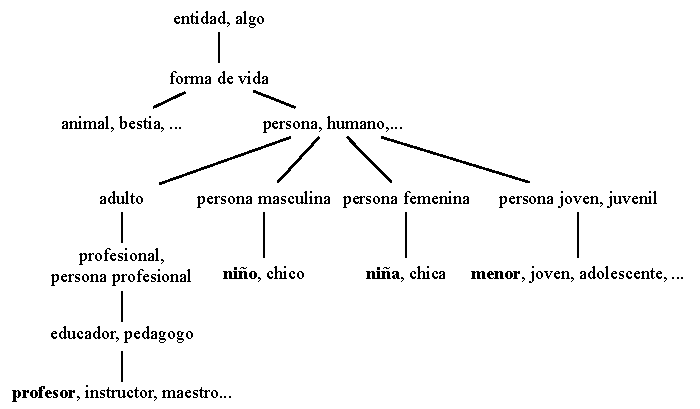
\includegraphics[width=0.7\linewidth]{../7_marco_teorico/imagenes/taxonomia_semantica}
		\label{fig:taxonomiasemantica}
	\end{figure}

	\begin{footnotesize}
		La similaridad entre palabras se define como \(S(w_1,w_2)=f(l,h),\)
		donde \(l\) es el camino más corto entre \(w_1\) y \(w_2\), y \(h\) es la profundidad del subsumidor de las mismas.
	\end{footnotesize}

	\framebreak

	Se define \(p(t)\) como la \textbf{probabilidad} de un concepto \(t\). Se entiende como:
	\[p(t)=\frac{freq(t)}{N},\]

	\bigskip

	Se define el \textbf{contenido de información} \(I(t)\) como:
	\[I(t)=-\log p(t).\]

	Entonces la \textbf{similaridad} entre dos términos \((i, j)\) se define como:
	\[S_R = I(ms(t_i,t_j)),\; (Resnik,\,1995)\]

	\[S_L(t_i, t_j)=\frac{2S_R(t_i,t_j)}{I(t_i)+I(t_j)}.\; (Lin\,et\,al.,\,1998)\]
\end{frame}

\begin{frame}
	\frametitle{Medidas de Similaridad}
	\textbf{Medidas de similaridad utilizadas}
	\bigskip
	\begin{itemize}[<*>]
		\item Term Frequency (TF)
		\item Term Frequency - Inverse Document Frequency (TF-IDF).
		\item Word2Vec
		\item FastText
		\item Semantic Distance
	\end{itemize}
\end{frame}

\begin{frame}
	\frametitle{Term Frequency (TF)}
	Caracteristicas de Term Frequency:
	\bigskip
	\begin{itemize}[<*>]
		\item También conocido en la literatura como \textit{Bag of words} (bolsa de palabras).
		\item Cada documento corresponde a un vector y cada término a una dimensión.
		\item El orden exacto de los términos es ignorado, pero se basa en el número de ocurrencias de cada uno de ellos en un documento.
		\item Se mide el grado de similaridad de dos documentos utilizando el coseno del ángulo entre dos vectores.
	\end{itemize}

	\bigskip
	\centering
	\textit{“Mary is quicker than John”} y \textit{“John is quicker than Mary”} \\
	\medskip
	\begin{scriptsize}
		(``Mary es más rápida que John'' y ``John es más rápido que Mary'')
	\end{scriptsize}
\end{frame}

\begin{frame}
	\frametitle{Term Frequency Inverse Document Frequency (TF-IDF)}
	Caracteristicas de TF-IDF:
	\bigskip
	\begin{itemize}[<*>]
		\item Se define \textit{document frequency} \(df_t\) como el número de documentos en una colección que contienen el término \(t\).
		\item \textit{Inverse document frequency}, o IDF: si un término de búsqueda se encuentra en muchos documentos, no es un buen discriminador, y se le debe asignar menor peso que a un término que se encuentra en pocos documentos.
	\end{itemize}

	\centering
	\[tfidf(t_i, d_j) = tf(t_i, d_j) \cdot idf(t_j)\]
\end{frame}

\begin{frame}
	\frametitle{Word2Vec}
	Características de Word2Vec:
	\bigskip
	\begin{itemize}[<*>]
		\item Modelos basados en redes neuronales con una capa oculta para computar representaciones de palabras como vectores.
		\item Las entradas y salidas de la red neuronal son palabras representadas como \textit{one-hot} vector.
		\item Los pesos de la capa oculta se van ajustando utilizando un clasificador de regresión Softmax.
		\item Estos pesos resultantes dan como resultado a la representación vectorial de las palabras de un vocabulario.
	\end{itemize}
\end{frame}

\begin{frame}
	Caracteristicas de FastText:
	\bigskip
	\frametitle{FastText}
	\begin{itemize}[<*>]
		\item Librería open-source desarrollada por Facebook.
		\item Utiliza un modelo sub-palabra.
		\item Cada palabra es representada como una bolsa de \textit{n-gramas}.
		\item Mayor precisión en diferentes medidas de rendimiento.
	\end{itemize}
\end{frame}

\begin{frame}
	\frametitle{Semantic Distance}
	Caracteristicas de Semantic Distance:
	\bigskip
	\begin{itemize}[<*>]
		\item La distancia semántica usada en este trabajo está basada en \textit{redes semánticas} y \textit{estadísticas de corpus} (Li et al., 2006).
		\item Enfocado en textos de distancia corta.
		\item Tiene en cuenta la \textit{información semántica} y la \textit{información del orden} de las palabras implicadas en las frases involucradas.
	\end{itemize}

	\begin{figure}
		\centering
		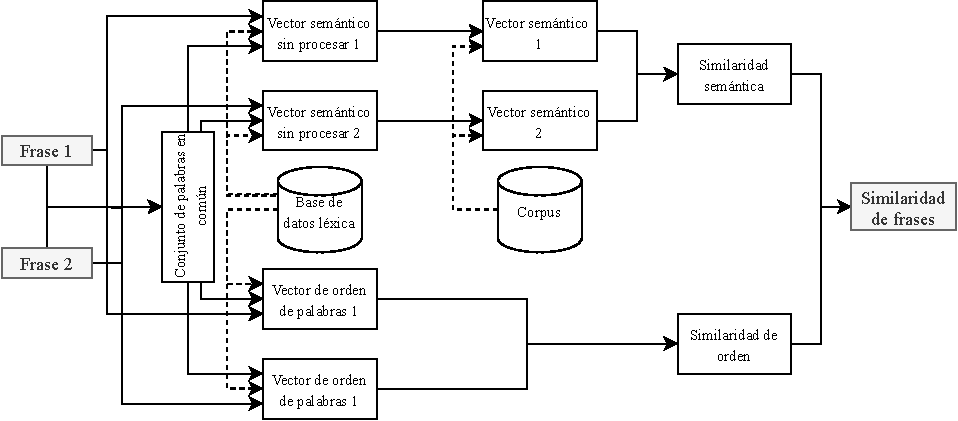
\includegraphics[width=0.7\linewidth]{../7_marco_teorico/imagenes/similaridad_sematinca_metodo}
		\label{fig:similaridadsematincametodo}
	\end{figure}
\end{frame}

\subsection{Ensamble de Clustering}
\begin{frame}
	\frametitle{Ensamble de Clustering}
	\begin{tcolorbox}[colback=blue!5,colframe=blue!40!black,title=Ensamble de Clustering]
		El \textit{Ensamble de Clustering} es un método para extraer clusters consistentes dadas particiones variadas de entrada.
	\end{tcolorbox}

 	\bigskip

	\begin{itemize}
		\item Combina resultados de distintos algoritmos de Clustering con clusters de distintas formas.
			\begin{itemize}[<*>]
				\item Distintos algoritmos de Clustering.
				\item Distintos parámetros para el mismo algoritmo.
				\item Distintas medidas de distancia.
			\end{itemize}
		\item Aprovecha la variabilidad agregada para encontrar una estructura \textit{inter-patrón}.
		\item Identificación de clusters subyacentes con formas, tamaños y densidades arbitrarias.
	\end{itemize}
\end{frame}

\begin{frame}
	\frametitle{Combinación de Evidencias}
	Toma la co-ocurrencia de pares de patrones en el mismo cluster a lo largo de las \(N\) particiones de datos para \(n\) patrones, para luego mapearlas a una \textit{matriz de co-asociación} \(n \times n\):
	\medskip
	\[C(i,j)=\frac{n_{ij}}{N},\]
	\medskip
	donde \(n_{ij}\) es el número de veces que el par de patrones \((i,j)\) es asignado al mismo cluster entre las \(N\) particiones de datos.

	\bigskip

	\textbf{Ejemplo}. \(N = 3\) particiones de datos.

\begin{figure}[!htb]
	\centering
	\begin{minipage}{.45\textwidth}
		\begin{figure}
			\centering
			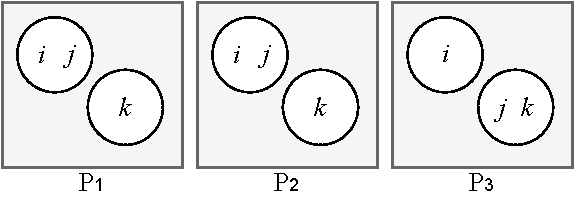
\includegraphics[width=0.9\linewidth]{3_marco_teorico/EAC}
		\end{figure}
	\end{minipage}%
	\begin{minipage}{.45\textwidth}
		\begin{scriptsize}
		\[  C(i,j)=\frac{2}{3} \Rightarrow  \begin{bmatrix}
			n_{11} 	& 	\dots 			   &     &  n_{1n} \\
			\vdots & 	n_{ij} = 2/3  & 	&  \\
			\vdots & 				          & \ddots 	&  \\
			n_{n1} &    					  & 	&  n_{nn}
		\end{bmatrix}\]
	\end{scriptsize}
	\end{minipage}
\end{figure}
\end{frame}
